The following sections are dedicated to the Base Station Layer of this project. This layer is dedicated to providing power to the Camera and Wireless Communication Layers autonomously through the Solar Battery Subsystem.

\subsection{Solar Battery Subsystem}

\begin{figure}[h!]
	\centering
 	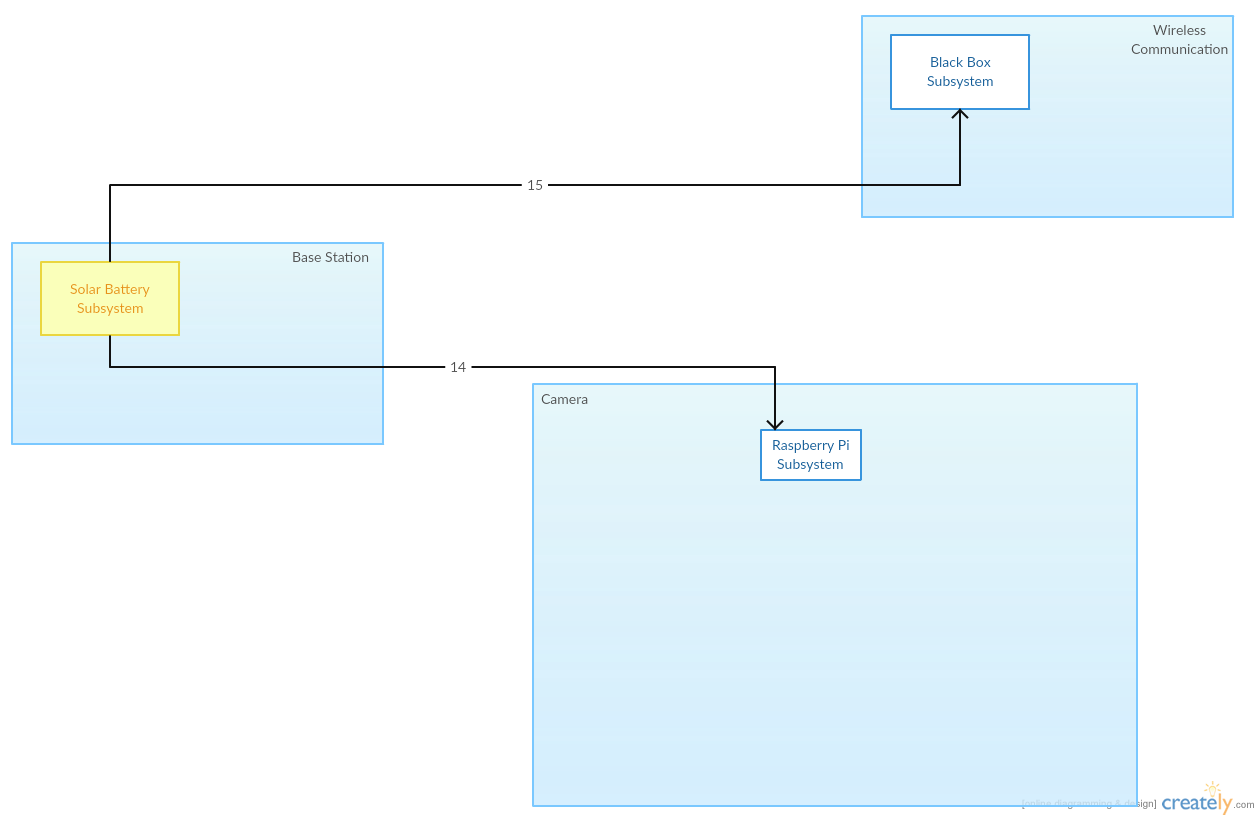
\includegraphics[width=0.60\textwidth]{images/ADSdiagrams/solarbatterysubsystem.png}
 \caption{Solar Battery description diagram}
\end{figure}

The above diagram illustrates graphically the interaction of the Solar Battery Subsystem with other Subsystems from the Wireless Communications Layer and the Camera Layer. 

\subsubsection{Assumptions}
The Solar Battery Subsystem is the second of two Subsystems that is necessary for this Architectural Design Specification but is provided entirely by TrafficNet LLC. Therefore it is assumed to be the responsibility of the vendor to provide.

\subsubsection{Responsibilities}
The Solar Battery provides the power supply for both the Wireless Communications Layer and the Camera Layer. Energy converted into 12V DC is supplied to the Raspberry Pi of the Camera Layer through a micro-USB port and similarly for the Black Box of the Wireless Communications Layer, vicariously powering all succeeding subsystems.

\subsubsection{Subsystem Interfaces}

\begin {table}[H]
\caption {Subsystem interfaces} 
\begin{center}
    \begin{tabular}{ | p{1cm} | p{6cm} | p{3cm} | p{3cm} |}
    \hline
    ID & Description & Inputs & Outputs \\ \hline
    \#15 & Interaction between Solar Battery and the Wireless Comunications Layer/bus & \pbox{3cm}{Solar Energy} & \pbox{3cm}{12V DC}  \\ \hline
    \#14 & Interaction between Solar Battery and the Camera Layer/bus & \pbox{3cm}{Solar Energy} & \pbox{3cm}{12V DC}  \\ \hline
    \end{tabular}
\end{center}
\end{table}
